\chapter{Model Fitting, Robust Estimation, and RANSAC}
\label{ch:lesson23}

Many computer vision problems boil down to fitting a model --- a line, a circle, a plane, a homography (Chapter~\ref{ch:lesson24}), a fundamental matrix --- to a set of corresponding points. In practice, that data almost always contains outliers: correspondences that are simply wrong. This chapter confronts that directly: least-squares fitting is catastrophically fragile to even a few bad points, and \textbf{RANSAC} is the standard fix.

\section{Ordinary vs.\ total least squares}

Fitting $y=mx+b$ by minimizing $\sum(y_i-(mx_i+b))^2$ --- \textbf{ordinary least squares (OLS)} --- measures error \emph{vertically}. That's the right choice when $x$ is known exactly and only $y$ is noisy, but not when both coordinates carry comparable noise, as they typically do for 2D image points: the fit gets biased toward whichever direction has less spread. \textbf{Total least squares (TLS)} instead minimizes the \emph{perpendicular} distance from each point to the line, treating both coordinates symmetrically.

For a 2D line, TLS needs no new machinery: the best-fit line passes through the centroid, and its direction is the eigenvector of the (centered) points' covariance matrix with the \emph{largest} eigenvalue --- exactly Chapter~\ref{ch:lesson06}'s covariance-and-eigenvectors idea, just picking out the axis of maximum spread instead of describing a blob's shape.

On a steep true line $y=3.00x+1.00$ with comparable noise on both axes: OLS fits $y=2.70x+1.67$ (biased, since $x$ is noisy too), while TLS fits $y=2.97x+0.98$ --- noticeably closer to the true slope, as Figure~\ref{fig:l23-1} shows.

\begin{figure}[h]
\centering
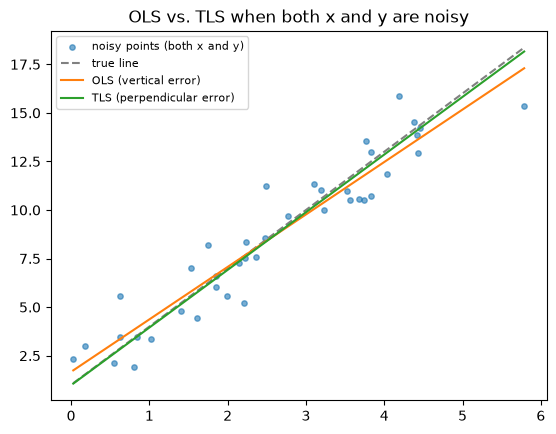
\includegraphics[width=0.55\textwidth]{figures/lesson23_fig01.png}
\caption{OLS (vertical error) vs.\ TLS (perpendicular error) when both $x$ and $y$ are noisy.}
\label{fig:l23-1}
\end{figure}

\section{Why least squares breaks under outliers}

Least-squares fitting minimizes the \emph{sum of squared} residuals. But squaring has a drawback: every outlier (point far from the model) contributes an enormous amount to the total error, causing the whole fit to move away from all the other, correct points. On data with 40 true inliers plus 15 unrelated outliers: the true line $y=2.00x+5.00$ becomes an OLS fit of $y=1.02x+9.81$ --- badly dragged off course, as Figure~\ref{fig:l23-2} shows.

\begin{figure}[h]
\centering
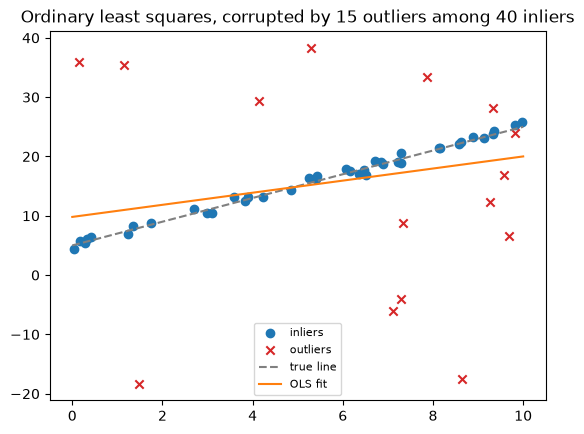
\includegraphics[width=0.55\textwidth]{figures/lesson23_fig02.png}
\caption{Ordinary least squares, corrupted by 15 outliers among 40 inliers.}
\label{fig:l23-2}
\end{figure}

\section{RANSAC: fit from the inside out}

\textbf{RANSAC} (RANdom SAmple Consensus, \citelink{fischlerbolles1981}{Fischler \& Bolles, 1981}) flips the strategy: instead of using \emph{all} the data and hoping outliers don't matter, it repeatedly picks the \emph{smallest possible} random subset needed to define a candidate model, counts how many of the remaining points agree with it (the \textbf{consensus set}), and keeps whichever candidate has the most agreement. A final least-squares refit on the winning inlier set gives the polished result.

On the same contaminated data: RANSAC fits $y=2.05x+4.94$, finding $42$ of $55$ points as inliers (planted: $40$ true inliers) --- essentially recovering the true line despite $27\%$ outlier contamination, as Figure~\ref{fig:l23-3} shows.

\begin{figure}[h]
\centering
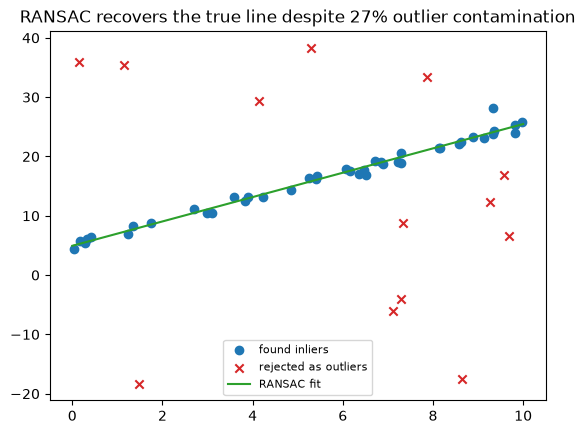
\includegraphics[width=0.55\textwidth]{figures/lesson23_fig03.png}
\caption{RANSAC's found inliers (blue) vs.\ rejected outliers (red), and the resulting fit.}
\label{fig:l23-3}
\end{figure}

\subsection*{How many iterations does RANSAC need?}

If a fraction $w$ of the data are inliers, and the model needs a minimal sample of $n$ points, the probability that any one random sample is entirely inliers is $w^n$. To be at least $p$ confident of drawing an all-inlier sample at least once across $N$ independent tries:
\begin{equation}
N = \frac{\log(1-p)}{\log(1-w^n)}.
\end{equation}

\begin{center}
\renewcommand{\arraystretch}{1.3}
\begin{tabular}{rrrr}
\hline
\textbf{Inlier \%} & \textbf{Line ($n{=}2$)} & \textbf{Homography ($n{=}4$)} & \textbf{Fund.\ matrix ($n{=}8$)} \\
\hline
90\% & 3  & 5   & 9 \\
70\% & 7  & 17  & 78 \\
50\% & 17 & 72  & 1{,}177 \\
30\% & 49 & 567 & 70{,}188 \\
\hline
\end{tabular}
\end{center}

Fitting a line only needs 2 points, so even fairly heavy contamination ($50\%$ outliers) needs just a few dozen iterations. Fitting a homography needs a minimal sample of 4 points, so the same inlier fraction needs an order of magnitude more iterations --- the price of a more complex model. A fundamental matrix (minimal sample 8) is far more sensitive still: at $30\%$ inliers, over $70{,}000$ iterations would be needed for the same confidence.

\section{A gentler alternative: robust loss functions}

RANSAC makes a hard inlier/outlier decision. An alternative family, \textbf{M-estimators}, instead reweights every point's contribution smoothly --- e.g.\ the \textbf{Huber loss} behaves like ordinary squared error for small residuals but switches to linear (much less aggressive) growth beyond a threshold, so a single very-wrong point can no longer dominate the total cost. RANSAC and M-estimators are complementary in practice: RANSAC is excellent at rejecting \emph{gross} outliers, while an M-estimator refinement afterward can down-weight smaller, more subtle deviations among the remaining inliers.

On the same data: OLS gives $y=1.02x+9.81$, Huber-reweighting gives $y=1.90x+5.58$, and RANSAC gives $y=2.05x+4.94$ --- Huber lands between the two, much closer to the true line ($y=2.00x+5.00$) than OLS, though not quite as exact as RANSAC on data this heavily contaminated, since a handful of gross outliers still pull a little on every iteration rather than being cut out entirely. Figure~\ref{fig:l23-4} compares all three fits.

\begin{figure}[h]
\centering
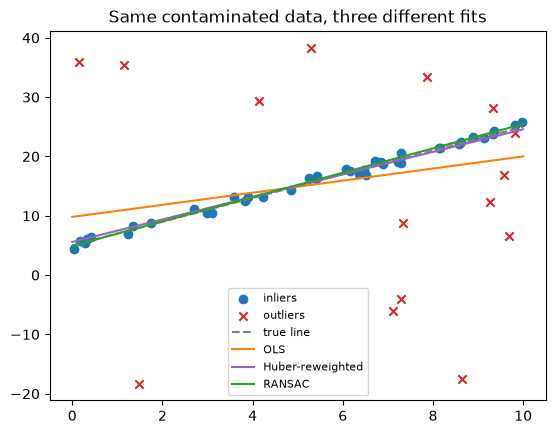
\includegraphics[width=0.55\textwidth]{figures/lesson23_fig04.png}
\caption{Same contaminated data, three different fits: OLS, Huber-reweighted, and RANSAC.}
\label{fig:l23-4}
\end{figure}

\subsection*{Exercises}
\begin{enumerate}
  \item Increase the outlier count until roughly $70\%$ of the points are outliers. Does 200 iterations remain enough to reliably recover the true line? Use the iteration-count formula to check whether 200 is even theoretically sufficient at that contamination level.
  \item Lower the RANSAC distance threshold from $2.0$ to $0.5$. Does the number of found inliers change, and why might too-strict a threshold actually start rejecting \emph{genuine} inliers?
  \item Try the Huber fit with a much smaller \code{delta} (e.g.\ $0.5$) and a much larger one (e.g.\ $5.0$). How does \code{delta} trade off between OLS-like behavior and RANSAC-like hard rejection?
\end{enumerate}

\vfill
\fullcode{lesson23}{lesson23_model_fitting_ransac}
